\documentclass{article} % For LaTeX2e
\usepackage{nips13submit_e,times}
\usepackage{hyperref}
\usepackage{url}
%\documentstyle[nips13submit_09,times,art10]{article} % For LaTeX 2.09


\usepackage{amsmath, amssymb, color}
%\usepackage{amsthm}
\usepackage{hyperref, url}
\usepackage{graphicx}               % Use pdf, png, jpg, or eps§ with pdflatex; use eps in DVI mode. TeX will automatically convert eps --> pdf in pdflatex



% New environment part
\newtheorem{definition}{Definition}
\newtheorem{assumption}{Assumption}
\newtheorem{fact}{Fact}
\newtheorem{theorem}{Theorem}%[section]
\newtheorem{lemma}[theorem]{Lemma}
\newtheorem{corollary}[theorem]{Corollary}
\newtheorem{proposition}[theorem]{Proposition}
\newtheorem{claim}[theorem]{Claim}
\newtheorem{remark}{Remark}
\newtheorem{example}{Example}
% Need the environment Proof ? Please use the following:
% {\noindent\bf Proof.}  ...........................  $\hfill \square$\\

% Bold type part.
\newcommand{\ba}{\mbox{\boldmath $a$}}
\newcommand{\bb}{\mbox{\boldmath $b$}}
\newcommand{\bc}{\mbox{\boldmath $c$}}
\newcommand{\bd}{\mbox{\boldmath $d$}}
\newcommand{\be}{\mbox{\boldmath $e$}}
\newcommand{\bff}{\mbox{\boldmath $f$}} %NOTICE!
\newcommand{\bg}{\mbox{\boldmath $g$}}
\newcommand{\bh}{\mbox{\boldmath $h$}}
\newcommand{\bo}{\mbox{\boldmath $o$}}
\newcommand{\bp}{\mbox{\boldmath $p$}}
\newcommand{\bq}{\mbox{\boldmath $q$}}
\newcommand{\br}{\mbox{\boldmath $r$}}
\newcommand{\bs}{\mbox{\boldmath $s$}}
\newcommand{\bt}{\mbox{\boldmath $t$}}
\newcommand{\bu}{\mbox{\boldmath $u$}}
\newcommand{\bv}{\mbox{\boldmath $v$}}
\newcommand{\bw}{\mbox{\boldmath $w$}}
\newcommand{\bx}{\mbox{\boldmath $x$}}
\newcommand{\by}{\mbox{\boldmath $y$}}
\newcommand{\bz}{\mbox{\boldmath $z$}}
\newcommand{\bzero}{\mbox
%{\Large 
{\boldmath $0$}}
%}

\newcommand{\bA}{\mbox{\boldmath $A$}}
\newcommand{\bB}{\mbox{\boldmath $B$}}
\newcommand{\bC}{\mbox{\boldmath $C$}}
\newcommand{\bD}{\mbox{\boldmath $D$}}
\newcommand{\bI}{\mbox{\boldmath $I$}}
\newcommand{\bM}{\mbox{\boldmath $M$}}
\newcommand{\bU}{\mbox{\boldmath $U$}}
\newcommand{\bV}{\mbox{\boldmath $V$}}
\newcommand{\bW}{\mbox{\boldmath $W$}}
\newcommand{\bX}{\mbox{\boldmath $X$}}
\newcommand{\bY}{\mbox{\boldmath $Y$}}
\newcommand{\bZ}{\mbox{\boldmath $Z$}}

\newcommand{\balpha}{\mbox{\boldmath $\alpha$}}
\newcommand{\bbeta}{\mbox{\boldmath $\beta$}}
\newcommand{\btheta}{\mbox{\boldmath $\theta$}}
\newcommand{\bgamma}{\mbox{\boldmath $\gamma$}}
\newcommand{\bdelta}{\mbox{\boldmath $\delta$}}
\newcommand{\bmu}{\mbox{\boldmath $\mu$}}
\newcommand{\bepsilon}{\mbox{\boldmath $\epsilon$}}
\newcommand{\blambda}{\mbox{\boldmath $\lambda$}}
\newcommand{\btau}{\mbox{\boldmath $\tau$}}
\newcommand{\bsigma}{\mbox{\boldmath $\sigma$}}
\newcommand{\bSigma}{\mbox{\boldmath $\Sigma$}}

% Specific math notation:
\newcommand{\real}[1]{\mbox{$\mathbb{R}^{#1}$}}
\newcommand{\prob}{\mbox{$\mathbb{P}$}}
\newcommand{\expect}{\mbox{$\mathbb{E}$}}
\newcommand{\var}{\mbox{$\mathbb{V}$}}
\newcommand{\compl}[1]{\mbox{$\mathbb{C}^{#1}$}}
\newcommand{\realN}[1]{\mbox{$\real{I_1 \times I_2 \times \dots \times I_{#1}}$}}
\newcommand{\complN}[1]{\mbox{$\compl{I_1 \times I_2 \times \dots \times I_{#1}}$}}
%\newcommand{\natural}{\mbox{$\mathbb{N}$}}

% Enumerate part
\newcommand{\V}[1]{\mbox{\boldmath $#1$}}
\newcommand{\RV}[1]{\mbox{\boldmath $\tilde{#1}$}}
\newcommand{\rv}[1]{\tilde{#1}}
\newcommand{\OPT}{{\mbox{OPT}}}
\newcommand{\SP}{{\tt{SP}}}
\newcommand{\CVX}{{\tt{CVX}}}
\newcommand{\LP}{{\tt{LP}}}
\newcommand{\D}{{\tt{D}}}
\newcommand{\ALG}{\tt{ALG}}
\newcommand{\cT}{{\cal T}}

%Added on Feb 23, 2015: Roman numbers, chapters, DEFINE format
\newcommand{\rmnum}[1]{\romannumeral #1} % Roman small letter
\newcommand{\Rmnum}[1]{\uppercase\expandafter{\romannumeral #1}} % Roman capital letter
\usepackage[raggedright]{titlesec}% 可换为 raggedleft  raggedright
\titleformat{\chapter}{\centering\Huge\bfseries}{Chapter \Rmnum{\thechapter} }{1em}{} % in book format
\newcommand{\df}{\bfseries \em}  % DEFINE format for text

%Added on April 30th, 2015: 
\usepackage{mathrsfs} %math-script format, then use \mathscr{F} 
\usepackage{enumerate} % change the symbols in enumerate
\graphicspath{{figures/}}  %图片路径

%Added on Jul 11th, 2015:
\newcommand{\tensorA}{\mbox{\boldmath $\mathcal{A}$}}
\newcommand{\tensorD}{\mbox{\boldmath $\mathcal{D}$}}
\newcommand{\tensorE}{\mbox{\boldmath $\mathcal{E}$}}
\newcommand{\tensorF}{\mbox{\boldmath $\mathcal{F}$}}
\newcommand{\tensorG}{\mbox{\boldmath $\mathcal{G}$}}
\newcommand{\tensorI}{\mbox{\boldmath $\mathcal{I}$}}
\newcommand{\tensorU}{\mbox{\boldmath $\mathcal{U}$}}
\newcommand{\tensorV}{\mbox{\boldmath $\mathcal{V}$}}
\newcommand{\tensorX}{\mbox{\boldmath $\mathcal{X}$}}
\newcommand{\tensorY}{\mbox{\boldmath $\mathcal{Y}$}}
\usepackage{multirow}
\usepackage{amsmath} 
\usepackage{stmaryrd}
\usepackage{float}
\usepackage{graphicx}
\usepackage{subfigure}
\usepackage{xcolor} 
\DeclareMathOperator*{\argmin}{argmin}

\usepackage{color}
\newcommand{\tbw}{\bigskip \mbox{\color{red} {\df (TBW) }}\bigskip}

\newcommand{\hide}[1]{}
\newcommand{\hao}[1]{{\color{red} [[Hao: #1]]}}



\newcommand{\hasPageBreak}{\newpage}
%\newcommand{\hasPageBreak}{}


% Added on Dec 8th, 2015: listings
\usepackage{listings}

% Added on March 9th, 2016: algorithm
\usepackage{algorithm} 
\usepackage{algorithmic}
\renewcommand{\algorithmicrequire}{\textbf{Input:}}
\renewcommand{\algorithmicensure}{\textbf{Output:}}





\title{Aiding Sentiment Evaluation with Social Network}


\author{
Pengfei Gao, Fan Yang, Hao Yin
\thanks{Each member contributes equally, and names are put in alphabetic order.} \\
Institute for Computational and Mathematical Engineering\\
Stanford University\\
Stanford, CA 94305 \\
\texttt{\{pfgao, fanfyang, yinh\}@stanford.edu}
}

% The \author macro works with any number of authors. There are two commands
% used to separate the names and addresses of multiple authors: \And and \AND.
%
% Using \And between authors leaves it to \LaTeX{} to determine where to break
% the lines. Using \AND forces a linebreak at that point. So, if \LaTeX{}
% puts 3 of 4 authors names on the first line, and the last on the second
% line, try using \AND instead of \And before the third author name.

\newcommand{\fix}{\marginpar{FIX}}
\newcommand{\new}{\marginpar{NEW}}

\nipsfinalcopy % Uncomment for camera-ready version

\begin{document}


\maketitle

\begin{abstract}
Some abstract
\end{abstract}


%!TEX root = report.tex

\section{Introduction}
%sentiment analysis
Sentiment analysis is one of the important tasks in natural language processing community[8] which helps people navigate the huge amount of user-generated content available online. Machine learning systems that make decision on the attitude of viewpoints to be positive, neutral or negative that enable people to understand the enormous body of opinions on the internet, ranging from product reviews to political positions. 

%challenge
One of the biggest challenges in sentiment analysis, as well as in almost all fields for natural language 
processing research, is the language variation. Words can mean different things to different people, 
and different people express their feeling and idea in a different way. However, such variation is believed
to be tractable from social factors [1]. For example, people of the same ago may speak in a
similar way [12] which might be influenced from their youth education, and people from the same community 
use the same language which is known as jargon. Therefore, social network information provides additional
information to solve the problem in language variable thus improve the general prediction performance
in natural language processing tasks.

%social network
Online social networks provide promising platforms to study the language variations. 
Most online websites have social network behind it, and user-generated content often appears in the context of social media. Therefore nowadays user-relationship information is now more easily obtainable. For example, huge amount of tweets from Twitter express people's opinions on different subjects. Each tweet is associated with a user and users formed social network structure through the mechanisms of ``follower''. When a user forms a link in the network such as Twitter, they tend to have a personal relationship then the principle in language called ``homophily'' suggests that users who are connected via some social relationship may also share similar opinions or linguistic variation (each community may have their own ``jargon'' in expressing ideas and sentiments). Figure 1 from [1] gives an example of how users from different communities may understand the word ``sick'' differently.

\begin{figure}[h]
\centering
\begin{minipage}{.5\textwidth}
  \centering
  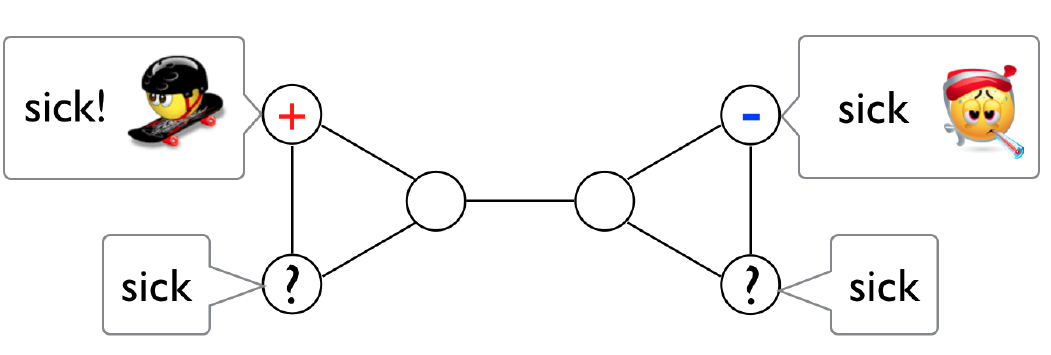
\includegraphics[width=1\linewidth]{sick}
    \label{fig:test1}
\end{minipage}%
\begin{minipage}{.5\textwidth}
  \centering
  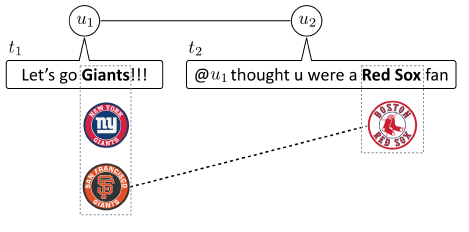
\includegraphics[width=1\linewidth]{Giant}
  
  \label{fig:test2}
\end{minipage}
\caption{Words such as ‘sick’ can express opposite sentiment
polarities depending on the author; Leveraging social relations for entity
disambiguation.}
\end{figure}


Nowadays, models that combine social network information with machine learning classification task are proposed in many literature. However, these models rarely utilize the state-of-art deep learning methods like convolutional neural network or network node embeddings which are common in social network and NLP communities. Previous research either use traditional machine learning methods to incorporate social network structure information as in [7] or they separate the textual and user information to build separate deep learning model as in [8]. None of the previous works directly model the interaction between author information, especially the social network information, and the sentence context. In this paper, we are going to explore different methods that utilize jointly social network information and textual information in sentiment analysis with one joint deep learning model that takes both social network information and textual information as input to classify the sentiment of sentences.

Our paper is structure as follows: section 2 will introduce related work to our task and how we relate them; section 3 will define the problem formally and introduce our dataset; section 4 will introduce our model and intuition; section 5 will demonstrate our numerical result; section 6 will discuss our result and draw our conclusion.


%!TEX root = report.tex
\section{Related Work}

\subsection*{Sentiment Analysis}

%cnn
The current state-of-the-art method is convolutional neural networks(CNN)[9] which takes word embeddings from sentences as inputs and output a softmax classification to identify sentence sentiment. The typical structure of such CNN is some convolutional layer on top of original sentence word embeddings, then a max pooling layer on top of the convolutional layer to extract some extreme information.  Finally, a dense layer with fully connected network is added to transform features from CNN to a softmax classifier. A simple CNN model with one convolutional layer of two-width window plus one max pooling layer with single channel can achieve amazing result[1]. Different initializations methods[11] could also be adopted to improve prediction accuracy, but they all share the similar structure as described above.


\subsection*{Network Node Embeddings}

To be added by Hao Yin ....


\subsection*{Aiding Classification with Social Network}

The intuition behind combing social network with classification is that users connected are more likely to hold similar opinions and use language similarly. 

Tan et al.(2011)[5] is the first paper to show social relationship information can be exploited to improve sentiment analysis. They have shown numerically that incorporating social-network information can indeed lead to statistically significant sentiment-classification improvements over the performance of a SVM baseline model that only has access to textual features. Yang and Eisenstein(2016)[1] is a more recent version for combining social network information and sentiment analysis. They study task for classifying sentiment to be positive, neutral and negative for each tweets given text and user ID information. Their model consider the author information and sentence information separately: each node (author) in the network is assigned an embedding vector using the LINE algorithm[2], and then is (softly) assigned each cluster on the network based on the embedding. Each cluster has its own model, which is a CNN model combined with max pool layer. Detail model specs are described in section 4 as a comparison to our model.

On the other hand, Yang and Chang(2016)[6] study another problems called entity linking, which is the task of identifying mentions
of entities in text, and linking them to entries in a knowledge base. They achieve the-state-of-art result with a tree-based model in Twitter data.  To further improve the performance, Yang et al.(2016)[7] propose to incorporate social network information in the same problem. Intuitively, socially linked individuals share interests, and are therefore likely to mention the same sorts of entities. Based on the previous the-state-of-art tree model[6], they build a bilinear model  that consider interactions of users and entities. This new model incorporating social network information has a F1 improvements of 1\%-5\% on benchmark datasets.

%!TEX root = report.tex

\section{Problem Definition and Data Description}
\label{Sec:ProblemData}


We obtained the data used by \cite{yang2017attention}. The data consists of a collection of tweets as well as some network information on Twitter. For each tweet sample, we have one tweet ID, one user ID, a sentiment label (positive, neutral, negative), and the tweet content itself. For example, the following are two examples of our data samples.
\begin{verbatim}
261140278944088066	17572408	negative	@USER may i have an industrial revolution ...
237571817550786563	727519172	neutral	@USER i told you shane would get his 5th-star ...
\end{verbatim}
We have three networks, i.e., FOLLOWER, MENTION and RETWEET network which have been explained in details by
\cite{yang2017attention}.


%!TEX root = report.tex

\section{Methodology}
\label{Sec:methodology}

%Methodology/Algorithm: What method or algorithm are you proposing? If there are existing implementations, will you use them and how? How do you plan to improve or modify such implementations?

Our project will start from the method proposed by Yang and Eisenstein(2016)[1], which is summarized in Figure \ref{Fig:Flow} (black lines). The model consider the author information and sentence information separately: each node (author) in the network is assigned an embedding vector using the LINE algorithm[3], and then is (softly) assigned each cluster on the network based on the embedding. Each cluster has its own model, which is a CNN model combined with max pool layer. This model provides a baseline in our project.

\begin{figure}[htbp] %  figure placement: here, top, bottom, or page
   \centering
   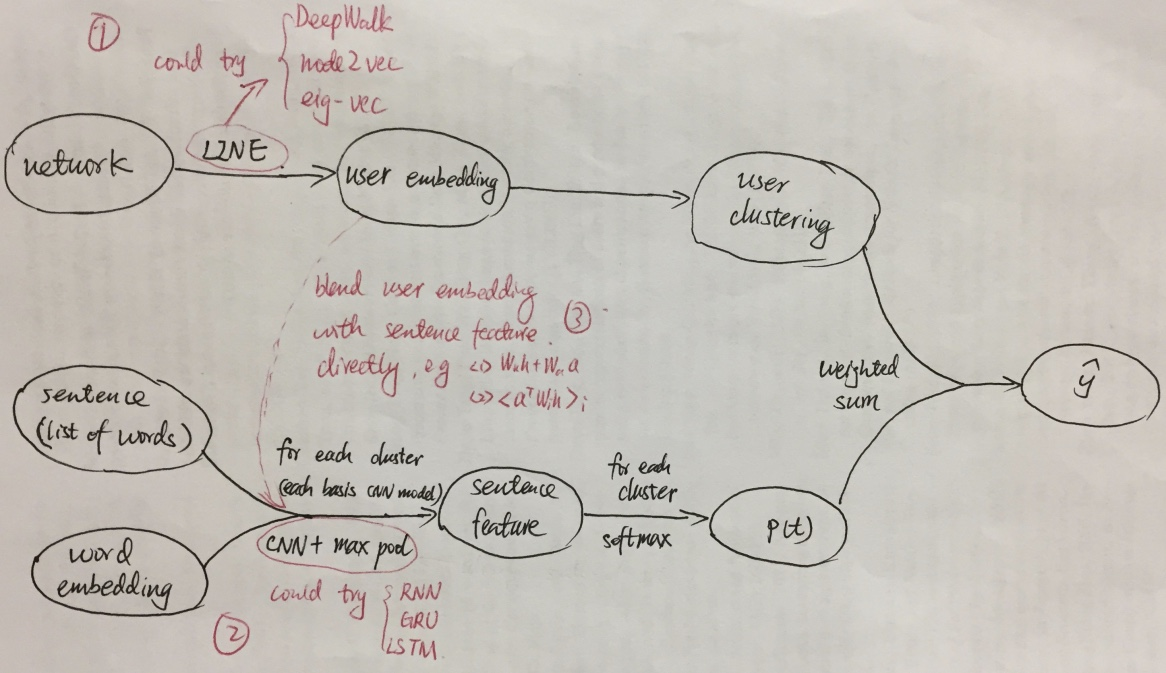
\includegraphics[width=5.2in]{flow.jpg} 
   \caption{General Methodology}
   \label{Fig:Flow}
\end{figure}



We are going to extend this model in three aspects, as is illustrated in the red lines in Figure \ref{Fig:Flow}. To be specific, 
\begin{enumerate}   [(1)]
%\setcounter{enumi}{3}
\item Using other node embedding methods in network analysis, such as \textit{DeepWalk}[2] and \textit{node2vec}[3];
\item Explore other methods to combine author information and sentence information, especially the bilinear form $a^T W h$ which measures the interaction between author and sentence. Here $a$ is the author embedding and $h$ is the sentence embedding.
\item Explore other models in sentiment analysis, such as RNN, GRU, and LSTM.
\end{enumerate}



%!TEX root = report.tex


\section{Experiments}



\begin{table}[htbp]
\begin{center}
\begin{tabular}{|c|c|c c c c|}
\hline
Embedding method & CNN & DeepWalk & LINE & node2vec & random\\
\hline
Dev2013  & 68.85 & 67.71 & \textbf{69.51} & 68.58 & 68.50 \\
\hline
Test2013  & 69.53 & 67.58 & \textbf{69.67} & 68.58 & 68.49 \\
Test2014  & \textbf{72.41} & 71.46 & 71.44 & 71.46 & 71.69 \\
Test2015  & 64.40 & \textbf{64.71} & 64.57 & 64.25 & 63.50 \\
\hline
Avg test sets & \textbf{68.78}& 67.92 & 68.56  & 68.10 & 67.89 \\
\hline
\end{tabular}
\end{center}
\caption{Prediction performance on each Dev and Test Sets. }
\label{Tb:}
\end{table}%



%!TEX root = report.tex

\section{Discussion and Conclusion}
Our experiment results are not cheerful, and we believe it is due to the following two reasons.
First, our sample size is too small, which makes the training suffer from overfitting. 
Even if we have employed different overfitting prevention techniques including $L_2$ 
penalty on weights, dropout, and early stop, considering that we only have 8,000 training tweet samples
it is not likely to build insightful models. We believe a larger training set would help solving this 
issue of overfitting.

Second, the experiment results show that the twitter networks are not informative in terms of language
variation. One follow another person does not mean that these two people are friends and should
have similar language usage preference. We believe a better network would be Facebook friendship network.

The experiment by Yang and Esteintin(2016)[1] is not persuasive either. We believe their model improvement is due to ensemble effect. In fact, in our running of their code, their baseline models outperform their social attention model.

Despite the unsatisfying result, we still believe social network information may help solving the issue of 
language variation and thus improve the general performance of sentiment analysis and other natural language tasks. 
Even though this user-activation method does not help the CNN baseline model, other ways of introduction may help, 
and may also help the prediction of other NLP models such as RNN and LSTM.


%!TEX root = report.tex

\section*{Reference}


























%\bibliographystyle{ormsv080} 
%\bibliography{Bibli}

\end{document}
